\documentclass[a4paper,11pt,dvipsnames, twocolumn]{article}
\setlength{\columnseprule}{0.3pt}
\usepackage[a4paper,left=1.5cm,right=1.5cm,top=1cm,bottom=1.5cm]{geometry}
\usepackage{amsmath,amsthm,amssymb,amsfonts}
% \usepackage{array}
\usepackage{booktabs}
\usepackage[table]{xcolor}
\usepackage{cuted}
\usepackage{xcolor}
\usepackage{graphicx}
\graphicspath{{./img/}}
\usepackage{setspace}
\newcommand*\diff{\mathop{}\!\mathrm{d}}
\newcommand*\Diff[1]{\mathop{}\!\mathrm{d^#1}}
\usepackage{enumitem}

\usepackage[utf8]{inputenc}
\usepackage[T1]{fontenc}
\usepackage[spanish]{babel}


\usepackage{tabularx}
\newcolumntype{Y}{>{\centering\arraybackslash}X}




\usepackage[locale=FR, per-mode=fraction, separate-uncertainty=true]{siunitx}
\usepackage{physics}
\AtBeginDocument{\RenewCommandCopy\qty\SI}

\usepackage{pgfplots}
\usepackage{adjustbox, tikz}
\usepackage{tikz-3dplot}
\usepackage{circuitikz}
% \usepackage{gnuplottex}

% \usepackage{ifpdf}
\ifpdf%
  \usepackage{pdftricks}
  \begin{psinputs}
    \usepackage{pst-optic}
%\usepackage{pstricks-add} 	
  \end{psinputs}
\else
  \usepackage{pst-optic}
  \newenvironment{pdfpic}{}{}
\fi
 

\usetikzlibrary{decorations}
\usetikzlibrary{decorations.pathmorphing}
\usetikzlibrary{shapes.geometric}
\usetikzlibrary{arrows}
\usetikzlibrary{arrows.meta}   %edg
\usetikzlibrary{calc}
\pgfplotsset{compat=newest}
\usetikzlibrary{patterns}

\def\cosa{-0.69466}
\def\sina{-0.71934}
% A custom arrowhead for use on x, y, z axes
\tikzstyle{axisarrow} = [-{Latex[inset=0pt,length=5pt]}]


\usepackage{pgffor}
\usepackage{readarray}

% --------------------------------------
% Formatting the header.
\def\M{30} % Number of columns in header.
\def\N{24} % Columns for questions (can be different to actual number of questions).
\def\P{6} % Columns reserved for Total.

% Number of questions and points.
% --------------------------------------


% % --------------------------------------
% % Data for questions.
% % Don't remove the '%' after \data{
% \def\data{%
% A 5.0 26 520 9.77 80
% B 2.4 26 520 6.50 70
% C 5.0 32 592 5.55 30
% D 6.0 32 592 4.44 30
% }
% \readarray\data\dataA[4,6] %read the data to \dataA
% % --------------------------------------


\usepackage[most]{tcolorbox}
% A style for tcolorbox without frame etc. "notcb"
\tcbset{notcb/.style={enhanced jigsaw, colback=white, coltitle=black,sharp corners, boxrule=0pt}}
% Style for the number tables
\tcbset{tabularheader/.style={arc=2pt,notcb,boxsep=0pt,left=0pt,colbacktitle=white,rounded corners=all,enhanced jigsaw,coltitle=black,tabularx={*{8}{Y|}Y},boxrule=1pt,attach boxed title to top left, boxed title style={enhanced jigsaw,sharp corners,left=0pt,boxrule=0pt}}}

\begin{document}

\pagenumbering{gobble}

% \foreach \j in {1,...,4} {

% Nombres y Apellido: el Código Civil y Comercial estableció el uso de un solo
% apellido, de cualquiera de los padres, y de manera opcional el del otro progenitor


\begin{strip} %place some material in full-width at any place on double-column page
  \vspace{-1.25cm}
\begin{tcolorbox}[colback=white]

\begin{tcbraster}[raster columns=4,raster equal height]
  \begin{tcolorbox}[notcb,fontupper=\bfseries\raggedright]
    {\Large \vphantom{y}Física II}\par
    2$^\circ$ 31
  \end{tcolorbox}
  \begin{tcolorbox}[raster multicolumn=2, notcb,fontupper=\bfseries\centering]
    % \centering
    {\Large \vphantom{y} Recuperatorio del 2\textsuperscript{do} parcial}\par
    28 de febrero de 2025
    % PARA REVISAR
  \end{tcolorbox}
  \begin{tcolorbox}[notcb,fontupper=\bfseries\raggedleft]
    \input{logoFRA_recortado}
    % 
\includegraphics[scale=0.2]{logoFRA_2022-recortado.png}
  \end{tcolorbox}
\end{tcbraster}
\begin{tcbraster}[raster columns=1, raster column skip=0pt, raster equal height,colback=white,before skip=0pt]
  \begin{tcolorbox}[coltitle=black,enhanced jigsaw,boxrule=0.5pt,boxsep=0pt,segmentation style={solid,black,line width=0.5pt},sidebyside,righthand width=9cm,fontupper=\tiny, fontlower=\tiny]
    Apellido
    \bigskip
    \tcblower
    Nombres
    \bigskip
  \end{tcolorbox}
\end{tcbraster}

\begin{tcbraster}[raster columns=\M, raster equal height,colback=white,before skip=0pt, boxsep=0.5pt]
  \begin{tcolorbox}[raster multicolumn=\N,tabularheader]
  % \begin{tcolorbox}[raster multicolumn=\N,tabularheader,title={\footnotesize some nice title}]
1 {\small ($2.5$ pts)}\par   \medskip\bigskip\bigskip & 2 {\small ($2.5$ pts)} & 3 {\small ($2.5$ pts)} & 4 {\small ($2.5$ pts)}
  %  1 (a) \par \bigskip\bigskip & 1 (b) \par  & 2 (a) \par  & 2 (b) \par  & 3 (a) \par  & 3 (b) \par & 4 \par 
  \end{tcolorbox}
  \begin{tcolorbox}[raster multicolumn=\P, colback=white,left=2pt,right=2pt]
    Nota

    \bigskip
    \bigskip
  \end{tcolorbox}
\end{tcbraster}

\end{tcolorbox}
% \textbf{Justificar todas las respuestas.} \hfill (\dataA[\j,1])
% \textit{Para alcanzar la condición de Aprobación con Final debe sumar 4 puntos o más en los problemas 1 a 4. Para alcanzar la condición de Aprobación Directa debe sumar 6 puntos o más en los problemas 1 a 4, y responder correctamente al menos 2 de las preguntas I a III. \textbf{Justificar todas las respuestas.}}
\end{strip}


\begin{enumerate}[wide, labelwidth=2pt, labelindent=0pt]
  % [leftmargin=*]


\item La figura muestra una espira cuadrada de lado $b=3.0\text{ cm}$, en el mismo plano que contiene un cable muy largo, y a una distancia $a=2.0\text{ cm}$ de dicho cable. Por el cable circula la corriente $i_1=5.0\text{ A}$ y por la espira la corriente $i_2=2.5\text{ A}$. Hallar el vector de la fuerza ejercida sobre el segmento $AB$ debida a la presencia del campo magnético generado por la corriente $i_1$.
\begin{center}
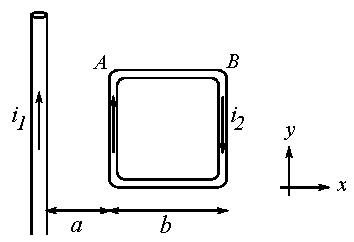
\includegraphics[scale=1]{2019_p3_fuerza_segmento.pdf}
\end{center}

\item Por un hilo rectilíneo de gran longitud circula una corriente variable en el tiempo, tal que su valor es:
\begin{align*}
    I(t) &=
    \begin{cases}
        0 & \text{si } t < 0\\
        at^2 - bt^3 & \text{si } 0 \leq t \leq 5\,\text{s}\\
        \dfrac{125}{6} & \text{si } 5\,\text{s} < t\\
    \end{cases}
\end{align*}
donde $a = \frac{5}{2}\,\text{A/s}^2$ y $b = \frac{1}{3}\,\text{A/s}^3$.
Junto al cable y coplanaria con él se encuentra una pequeña espira de área igual a $2\,\text{cm}^2$, con su centro situado a $20\,\text{cm}$ de distancia del hilo. Encuentre el valor de la fem inducida en la espira en el instante $t = 2\,\text{s}$, asumiendo que el campo magnético es uniforme sobre el área de la espira. 

\item Calcule las corrientes $I_1$, $I_2$ e $I_3$ que se indican en el circuito de la figura.
\begin{center}
  \begin{circuitikz}[scale=1]
    \def\sep{1.3}
    \draw (0,0) to[R=$\SI{10.00}{\ohm}$, color=red] (7,0)
    (0,\sep) to[battery2, l=$\SI{12.00}{\volt}$, color=cyan] (1.5,\sep) to[R=$\SI{1.00}{\ohm}$, color=red] (3.5,\sep) to[R=$\SI{1.00}{\ohm}$, color=red] (5.5,\sep) to[battery2, invert, l=$\SI{9.00}{\volt}$, color=cyan] (7,\sep)
    (0,2*\sep) to[R=$\SI{5.00}{\ohm}$, color=red] (3.5,2*\sep) to[R=$\SI{8.00}{\ohm}$, color=red] (7,2*\sep)
    (0,0) -- (0,2*\sep)
    (7,0) -- (7,2*\sep)
    (3.5,\sep) -- (3.5,2*\sep);
    \draw[<-,blue!50!black, thick] (4,-0.4) -- (3,-0.4) node[midway,below=1] {$I_3$};
    \draw[<-,blue!50!black, thick] (5.5,\sep-0.4) -- (4.5,\sep-0.4) node[midway,below=1] {$I_1$};
    \draw[<-,blue!50!black, thick] (1.5,\sep-0.4) -- (2.5,\sep-0.4) node[midway,below=1] {$I_2$};
  \end{circuitikz}
\end{center}



\item El circuito de la figura se encuentra funcionando en régimen estacionario, con la llave cerrada. La capacidad del capacitor es $C = \SI{3.5}{\milli\farad}$, el valor de las resistencias es $R_1 = R_2 = R_3 = \SI{250}{\ohm}$, y la diferencia de potencial en la batería es $\varepsilon = \SI{32}{\volt}$. Si en un cierto instante se abre la llave, calcule la corriente que circulará a través de $R_3$, $\SI{1}{\second}$ después de abrir la llave, e indique el sentido de circulación de esa corriente. 

%
\begin{center}
  \begin{circuitikz}[scale=1]
      % \draw (0,0) to[switch, l=$S_2$] (4,0) -- (4,3)
      % (0,1.5) to[R=$R$, color=red] (2,1.5) to[L, l=$L$, color=green!80!black] (4,1.5)
      \draw (1.5,0) -- (2,0) to[battery2, l=$\varepsilon$] (3.5,0)
      to[R=$R_2$] (5,0) -- (5.5,0) -- (5.5,1.5);
      \draw (0,0.75) to[switch] (1.5,0.75);
      \draw (5.5,0.75) -- (6,0.75);
      \draw (0,-1.25) -- (0,2.75)
      to[C, l=$C$] (6,2.75) -- (6,-1.25);
      \draw (1.5,0) -- (1.5,1.5) to[R=$R_1$] (5.5,1.5); 
      \draw (0,-1.25) to[R=$R_3$] (6,-1.25); 
  \end{circuitikz}
\end{center}
  


\end{enumerate}

\end{document}
